\documentclass[11pt]{report}
\usepackage[german,english]{babel}

%\documentclass[english, 10pt]{report}
\usepackage{amssymb}
\usepackage{babel}
\usepackage{caption}
\usepackage{courier}
\usepackage{epstopdf}
\usepackage{fancyhdr}
\usepackage[T1]{fontenc}
\usepackage{geometry}                % See geometry.pdf to learn the layout options. There are lots.
\usepackage{graphicx}
\usepackage{hyperref}
%\usepackage[latin9]{inputenc}
\usepackage[utf8]{inputenc}
\usepackage{listings}
\usepackage{moreverb}
\usepackage{multirow}
%\usepackage[parfill]{parskip}    % Activate to begin paragraphs with an empty line rather than an indent
\usepackage{verbatim}
\usepackage{xcolor}


\geometry{a4paper}                   % ... or a4paper or a5paper or ... 
%\geometry{landscape}                % Activate for for rotated page geometry

%
% Listings to view code
%
 \lstset{
         basicstyle=\footnotesize\ttfamily, % Standardschrift
         numbers=left,               % Ort der Zeilennummern
         numberstyle=\tiny,          % Stil der Zeilennummern
         %stepnumber=2,               % Abstand zwischen den Zeilennummern
         numbersep=5pt,              % Abstand der Nummern zum Text
         tabsize=2,                  % Groesse von Tabs
         extendedchars=true,         %
         breaklines=true,            % Zeilen werden Umgebrochen
         keywordstyle=\color{red},
    		frame=b,         
 %        keywordstyle=[1]\textbf,    % Stil der Keywords
 %        keywordstyle=[2]\textbf,    %
 %        keywordstyle=[3]\textbf,    %
 %        keywordstyle=[4]\textbf,   \sqrt{\sqrt{}} %
         stringstyle=\color{white}\ttfamily, % Farbe der String
         showspaces=false,           % Leerzeichen anzeigen ?
         showtabs=false,             % Tabs anzeigen ?
         xleftmargin=17pt,
         framexleftmargin=17pt,
         framexrightmargin=5pt,
         framexbottommargin=4pt,
         %backgroundcolor=\color{lightgray},
         showstringspaces=false      % Leerzeichen in Strings anzeigen ?        
 }
 \lstloadlanguages{% Check Dokumentation for further languages ...
         %[Visual]Basic
         %Pascal
         %C
         C++
         %XML
         %HTML
         %Java
 }
    %\DeclareCaptionFont{blue}{\color{blue}} 

  %\captionsetup[lstlisting]{singlelinecheck=false, labelfont={blue}, textfont={blue}}
\DeclareCaptionFont{white}{\color{white}}
\DeclareCaptionFormat{listing}{\colorbox[cmyk]{0.43, 0.35, 0.35,0.01}{\parbox{\textwidth}{\hspace{15pt}#1#2#3}}}
\captionsetup[lstlisting]{format=listing,labelfont=white,textfont=white, singlelinecheck=false, margin=0pt, font={bf,footnotesize}}
%
% End Listings
%

\begin{document}

\rhead{
\includegraphics[scale=.9]{picturesPublic/logoHTL.png}}
\cfoot{}
\begin{titlepage}
\thispagestyle{fancy}

\begin{center}

\vspace*{8em}

{\LARGE Diploma Thesis}

\vspace{2em}

{\large H\"ohere Technische Bundeslehranstalt Leonding \\[.5em]
Abteilung f\"ur EDV und Organisation}

\vspace{8em}

{\Huge High Level Movement Control for Autonomous Vehicle}
\end{center}

\vspace{18em}

Submitted by: {\bf Andreas Gruber, 5BHDVK} \\[.5em]

Date: {\bf \today} \\[.5em]

Supervisors: {\bf Peter Bauer, Roland Richter}
\end{titlepage}
\section*{Declaration of Academic Honesty}
Hereby, I declare that I have composed the presented paper independently on my own and without any other resources than the ones indicated. All thoughts taken directly or indirectly from external sources are properly denoted as such.

This paper has neither been previously submitted to another authority nor has it been published yet. \\[1em]
Leonding, October 6, 2012 \\[5em]
Andreas Gruber \\[5em]

%\begin{otherlanguage}{german}
\section*{Eidesstattliche Erklärung}
Hiermit erkläre ich an Eides Statt, dass ich die vorgelegte Diplom- / Bachelor- / Masterarbeit selbstständig und ohne Benutzung anderer als der angegebenen Hilfsmittel angefertigt habe. Gedanken, die aus fremden Quellen direkt oder indirekt übernommen wurden, sind als solche gekennzeichnet.

Die Arbeit wurde bisher in gleicher oder ähnlicher Weise keiner anderen Prüfungsbehörde vorgelegt und auch noch nicht veröffentlicht. \\[1em]
Leonding, am 6. Oktober 2012 \\[5em]
Andreas Gruber
%\end{otherlanguage}
\begin{abstract}
The amount of robots in our life rises very fast.
They build our cars, they mow the lawn, they do the hoovering and a lot of other things which most people do not even recognize.
Most of these intelligent systems which are mobile systems, are connected to a central control
station or are remotely controlled. In some cases, however, it is
impossible to connect the mobile system to a control device or the
mobile system needs to act very fast and, therefore, needs to calculate
its behaviour by its own. In this case a device needs to know  its
current position, speed, and direction. Also a lot of other properties
need to be known to compute a behaviour which is as good as possible
for the current situation. To find out the values of these properties
the robot needs a lot of sensors. In order to keep the production
costs low, the mass of these sensors is pretty cheap which, in turn,
rises the problem that those can produce errors and they even can
brake while the device is working. In one of these cases the device
should detect that the sensor doesn't work any more and replace its
results by the result of other sensors.

The main goal of this thesis is to build a system which calculates the
most accurate current position of a model car based on a set of different
(cheap) sensors. To take more cheap sensors has a lot of pros. First the whole device can be produced very cheaply.
Another very important consequence is that other cheap sensors help
to improve the results. The most important advantage is that %This can be improved
errors and measuring faults can be detected and the wrong values can
be replaced by correct ones. Systems like this have a big application
spectrum in future because autonomous robots will be needed in more
and more branches.
\end{abstract}

%Write about three sentences about the co-operation with FLLL in Hagenberg.
%\begin{itemize}
%\item There is a co-operation, who is the contact person
%\item What is the FLLL working in?
%\item What is the general project you are working in? How does your thesis
%fit into the general work of the FLLL?\end{itemize}

\begin{otherlanguage}{german}
\begin{abstract}

\end{abstract}
\end{otherlanguage}
\tableofcontents
\chapter{Environment} \label{chap:environment}
\section{Introduction} \label{sec:introduction}
In this chapter the setup of the autonomous vehicle is presented. 
Here all microcontroller which were cousidered to be used are listed.
Also the main usage of most of them are shown.
Another topic of this chapter is an introduction to the environment of Arduino.
Last but not least the different types of sensors are shown.

\section{AVR} \label{sec:AVR}
In this section all informations and pictures are taken from \cite{web:Atmel} otherwise it is described separately.

AVR is the name of a microcontroller-family which is produced by the company Atmel.
Atmel currently produces different types of microcontrollers.
These types can be grouped in:

\begin{itemize}
\item 32-bit AVR UC3
\item AVR XMEGA
\item Automotive AVR
\item megaAVR
\item tinyAVR
\end{itemize}

These families differ in size of memory, clock rate and the supply voltage which is need from the controller.
As example the tinyAVR also known as ATtiny is a very small cheap microcontroller which only need a power supply down to 0,7 V.
Beside these listed chips there are yet another which handle battery management.
In addition to AVR Atmel also produces other chip-families.
For details we refer to \url{ http://www.atmel.com/products/microcontrollers/avr/default.aspx }

For this thesis mostly megaAVR also known ATmega are used because this are the most popular and so they are used on the arduino boards.
These boards are shown in \ref{sec:arduino}.

\subsection{ATmega~2560} \label{sec:atmega2560}
In this section all informations and pictures are taken from \cite{manual:atmega2560}.

This information 
We start with a brief description of the AVR microcontroller which is used on the Arduino~Mega~2560 boards.
These boards will be shown in \ref{sec:arduino}
ATmega~2560 is part of many different electronic projects.
It is a very many-sidet microcontroller because has a lot of different hardware implemented features.
This chip contains a lot of input and output interfaces so it can communicate with other chips without wasting invaluable computing time.
Another advantage of these hardware implemented I/O interfaces is that no code have to be written .

In the following the main technical features will be summarized:
\subsubsection{Summary} \label{sec:atmega2560Summary}
\begin{tabular}{ll}
Speed Grade	& 0-16 MHz	\\
Flash Memory	& 256 KB	\\
SRAM			& 8 KB	\\
EEPROM		& 4 KB	\\
I/O Lines		& 86		\\
8-bit Timer		& 2		\\
16-bit Timer	& 4		\\
4-bit PWM		& 4		\\
2 to 16-bit PWM	& 12		\\
10-bit ADC		& 16		\\
USART / UART	& 4		\\
TWI / I2C		& 1		\\
\end{tabular}


\section{Arduino} \label {sec:arduino}
In this section all informations and pictures are taken from \cite{web:arduino} otherwise it is described separately.

The term Arduino stand for a full environment to program different microcontroller.
All parts of the Arduino environment are a open source. 
On part of this environment are the Arduino-Boards.
These boards differs in size, functions, prize, ... .
On each board there is the full hardware to program and run the microcontroller.
So a USB to serial converter is installed on-board.
Most boards also contains a voltage regulator to feed it by an external power supply too and a circuit to switch to the USB power supply.
At least each boar contain a button to reset the microcontroller.

Another Part of the Arduino environment is the Arduino software.
With this software it is possible to compile c++ code with the avr-gcc compiler which is part of the GNU Compiler Collection.
This software can also transfer the compiled sketch to the USB to serial converter and this chip programs the microcontroller.

The most useful part of the Arduino environment is the library.
This library contains code to address the pins.
In result of that the sketch code is more compact and so it is easier to read the code.
The result of this is that the amount of bugs are reduced.


\subsection{Arduino Shields} \label{sec:arduinoShields}
Shields are boards which have the design that they can be plugged on top of the Arduino.
Those shields are used to extend the Arduinos capabilities.
Most shields are designed for the Arduino~UNO but the design of the Arduino~Mega is compatible for most of the shields of the Arduino~UNO.
But this is not a backward compatibility. Shields for the Arduino~Mega does not fit on a Arduino~UNO.
Examples for Arduino Shields are:
\begin{itemize}
\item MotorDriver Shields
\item GPS Shields
\item Memory Shields
\item Display Schields
\end{itemize}


\subsection{Arduino~Mega~2560} \label {sec:arduinoMega2560}
\begin{figure}
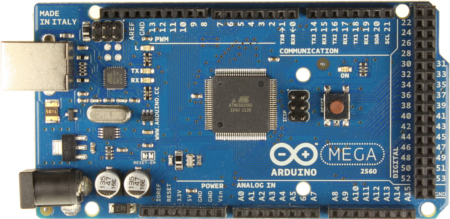
\includegraphics[scale=0.5]{picturesArduino/arduinoMega2560_R3_Front.jpg}
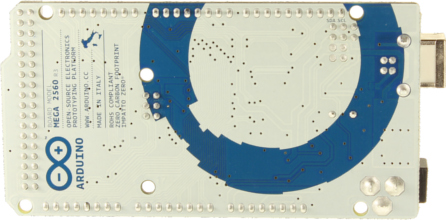
\includegraphics[scale=0.5]{picturesArduino/arduinoMega2560_R3_Back.jpg}
\caption{Board of the Arduino Mega 2560}
\label{fig:mega2560}
\end{figure}

The Arduino~Mega~2560 is a microcontroller board based on the ATmega~2560.
Basically this is a board holding an ATmega~2560 so the technical features from the ATmega~2560 are also applicable for the Arduino~Mega~2560.
See figure~\ref{fig:mega2560} for an image of this microcontroller.
% and adding some convenient features to plug in extra...

%The design of the Arduino Mega has the advantage that it is backward compatible to the Arduion UNO controller. In particlular the shields
%(see section~\ref{sec:arduinoShields} for details) from the Arduino UNO are compatible with the Arduino Mega.


\subsection{Datatypes} \label {sec:datatypes}
Here the data types of AVRs are described because they differ significantly from the sizes normally used on ``regular'' PCs.
One example is the type int which only has a size of 2 bytes instead of 4 bytes like on an PC.
Another very interesting types are floating-point numbers. 
On AVRs floating-point calculations have some significant characteristics.
A very interesting fact is that floating-point calculations are much slower than integer calculations.
Also the precision of floating-point calculations differs from usual PCs.
On a PC a float has a size of 4 bytes and a double has a size of 8 bytes.
On AVRs a double is as large as float and has 4 bytes in result of this fact the usual precision are 6-7 digits.
See table~\ref{tab:datatypes} for details.

\begin{table}
{\large
\begin{center}
\begin{tabular}{|l|r|r|r|}
\hline
\multirow{2}{*}{data type} & \multirow{2}{*}{Bit} & \multicolumn{2}{|c|}{value}  \\
\cline{3-4}
& & min & max \\
\hline
int8\_t, signed char				& $8$	& $-2^{7}$		& $2^{7}-1$	\\
int16\_t, signed short, signed int		& $16$	& $-2^{15}$		& $2^{15}-1$	\\
int32\_t, signed long				& $32$ 	& $-2^{31}$		& $2^{31}-1$	\\
int64\_t, signed long long			& $64$ 	& $-2^{63}$		& $2^{63}-1$	\\
& & & \\
uint8\_t, unsigned char			& $8$	& $0$			& $2^{8}-1$	\\
uint16\_t, unsigned short, unsigned int	& $16$ 	& $0$ 			& $2^{16}-1$	\\
uint32\_t, unsigned long			& $32$ 	& $0$			& $2^{32}-1$	\\
uint64\_t, unsigned long long		& $64$ 	& $0$			& $2^{64}-1$	\\
& & & \\
float, double					& $32$ 	& $-3.4028235*10^{38}$	& $3.4028235*10^{38}$	\\
\hline
\end{tabular}
\end{center}
}
\caption{Sizes of data types on the AVR}
\label{tab:datatypes}
\end{table}


\subsection{Microcontroller I/O} \label{sec:microcontrollerIO}
In this section the interface to the Arduinos I/O is described.
First the basic analog and digital I/O is shown.
This is followed by a description of the UART API. 
Finally the I2C is described.
For the more complex parts of the I/O we give small code snippets to illustrate the programming of the I/O!


\subsubsection{Input Pins:} \label{sec:inputPins}
The following instruction describe how a value can be read from a pin.
\begin{itemize}
\item First the pin have to be set as an input pin.\\
\lstinline|pinMode(pin, INPUT);|

\item Then the internal pull up Resistor can either on or off.\\
Turn on:\\
\lstinline|digitalWrite(pin, HIGH);|\\
Turn off:\\
\lstinline|digitalWrite(pin, LOW);|\\

\item If the microcontroller has the right settings the pin can be read.
One possibility is to read a digital value.
This return False if the voltage is lower than 2 volts and True if the voltage is above 3 volts.
If the voltage is between 2 and 3 volts either True or False can be returned.
In this case the result can be random.\\
\lstinline|value = digitalRead(pin);|\\
The other possibility is to read an analog value.
This return a value with a resolution of 10 Bit.
So it will return a value between 0 and 1024.
0 stand for 0 v and 1024 stand for 5V.\\
\lstinline|value = analogRead(Apin)|\\
\end{itemize}

\subsubsection{Digital Output Pins}\label{sec:digitalOutputPins}
The digital output of the Arduinos ports can be used to send data or switch some components off and on.
Very interesting is that the the high output voltage is lower than the supply voltage and the low output voltage is higher than the supply voltage.
This is because the transistors inside the IC have a small voltage drop.
Before the digital output pins can be used the pinmode have to be set to output:\\
\lstinline|pinMode(pin, OUTPUT);|\\
To write a low voltage on the port this code line have to be executed:\\
\lstinline|digitalWrite(pin, LOW);|\\
This code line write a high voltage on the port:\\
\lstinline|digitalWrite(pin, HIGH);|\\


\subsubsection{Analog Output Pins - PWM}\label{sec:analogOutputPinsPWM}
\begin{figure}
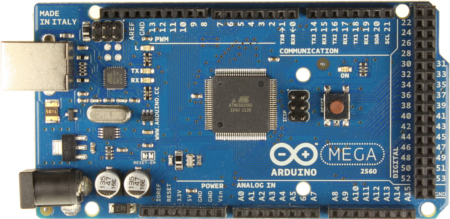
\includegraphics[scale=0.5]{picturesArduino/arduinoMega2560_R3_Front.jpg}
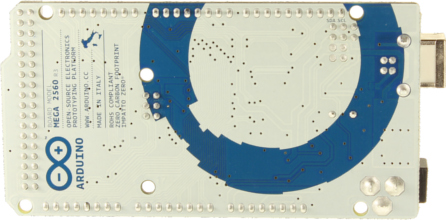
\includegraphics[scale=0.5]{picturesArduino/arduinoMega2560_R3_Back.jpg}
\caption{Board of the Arduino Mega 2560}
\label{fig:pwm}
\end{figure}

Before the code to set an analog voltage on the output pin is shown PWM have to be explained.

PWM which stand for pulse width modulation is one of many methods to produce a analog voltage.
The main thing to know that PWM in the strict sense doesn't make a real analog voltage.
In truth PWM switch the pin frequently on and off. 
The most electronic components allow to give the input via PWM as example almost all motor drivers.
If a real analog signal required smoothing capacitors can be used.
This will return a real analog voltage.
See figure~\ref{fig:pwm}.

The resolution of the PWM pins are 8 bit so the minimal value is 0 which equates to the low level voltage and the maximal value is 255 which equates the high level voltage. 
To output a PWM signal the port has to be set as output. See section~\ref{sec:digitalOutputPins}.
Then the following code line can be executed.\\
\lstinline|analogWrite(PWMpin, value);|


\subsubsection{UART}\label{sec:uart}
The term UART means Universal Asynchronous Receiver Transmitter also known as RS-232.
UART is a serial interface and it is one of the most important on PCs and microcontroller.
Today in regular new PC the RS-232 interfaces are out of date because the USB have suppressed the RS-232.
To convert from from the serial interface USB to the serial interface RS-232 there exists several ICs like the CP2102.
Another possibility to convert this serial interfaces is to program a microcontroller to an converter like it is realized on the Arduino.
On the Arduino~Mega~2560 the USB to serial interface is programmed on a ATmega16u2.

To use the UART on the Arduino the following code has to be executed.\\
Before the serial connection is used it has to be started: \\
\lstinline|Serial.beginn(speed);| \\
Then date which have a size of one byte can be written to the serial port.
If there is more than one byte this method have to be called for each byte: \\
\lstinline|Serial.write(value);| \\
Or something can be printed the serial port. 
This can be used instead of Serial.write:\\
\lstinline|Serial.println(value);| \\

A small code snippet for a serial connection could look like this:\\
\begin{lstlisting}
Serial.beginn(9600);
Serial.println("Hello World");
byte in;
while(Serial.available() > 0)
	in = Serial.read();
char c = Serial.read();
\end{lstlisting}


\subsubsection{I2C}\label{sec:i2c}
The I2C bus is also a serial bus like UART with the difference that I2C uses a master and slave administration.
Another difference is, that more then two devices can be joined to the I2C bus.
The address has 7 bits and so it can be set from 0 to 127.
In result of that the maximal number of devices is 128.

To use the I2C bus on the Arduino the following code has to be executed.\\
At first the I2C bus has to be started: \\
\lstinline|Wire.beginn(address);| \\
Then a request can be started: \\
\lstinline|Wire.requestFrom(device,size);| \\
At least one byte can be read from the device.
If the manual of the device say that there is more than one byte this method can be executed more than once. \\
\lstinline|byte b = Wire.read();| \\
Another option is to start a transmission:\
\lstinline|Wire.beginTransmission(device);| \\
Then it is possible to write data to the communication partner:\\
\lstinline|Wire.write(value);|\\
After sending the data the transmmission have to be closed:\\
\lstinline|Wire.endTransmission();|\\
An example for an I2C connection could look like this:\\
\begin{lstlisting}
Wire.begin()
Wire.requestFrom(0x23,1);
byte b = Wire.read();
Wire.beginTransmission(0x23);
Wire.write(b);
Wire.endTransmission();
\end{lstlisting}



\chapter{Positioning}
\begin{table}
{\large
\begin{center}

Sensor Types\\
\begin{itemize}
\item absolute sensors
	\subitem lateration
		\subsubitem GPS	
	\subitem environment detection
		\subsubitem camera
		\subsubitem bumper
\item relative sensors
	\subitem touchless
		\subsubitem gyro sensor
		\subsubitem acceleration
		\subsubitem magnetometer
	\subitem other
		\subsubitem rotary encoder
		\subsubitem mouse sensor
%	\begin{itemize}
%	\item test
%	\end{iitemize}
\end{itemize}

\begin{tabular}{|l|}
\hline
Sensor Name\\
\hline

\hline
\end{tabular}
\end{center}
}
\caption{Sizes of data types on the AVR}
\label{tab:positioningSensors}
\end{table}



\bibliography{bibliography}{}
\bibliographystyle{plain}

\end{document}